\chapter{Ingénierie des exigences}
\section{Approche Top-Down}

Dans cette partie nous allons analyser notre système avec une approche Top-Down. Cela signifie que nous adopterons une démarche de conception descendante. Pour cela nous avons tracé le diagramme "bête à cornes", que l'on peut voir sur la figure \ref{fig:beteacorne}. Il permet de représenter graphiquement l'expression du besoin. Comme on peut le voir sur le diagramme, le système BMONS rend service aux apiculteurs en agissant sur une ou plusieurs ruches. Il a pour but d'aider la surveillance d'un rucher et d'avertir l'apiculteur en cas de problème.


\begin{figure}[h!]
\centering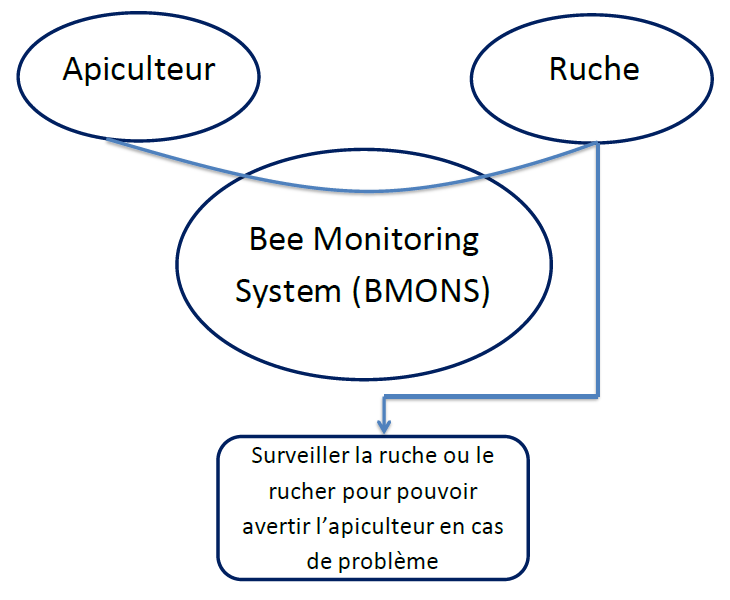
\includegraphics[scale=0.5]{BeteACornesBMONS.png}
\caption{\label{fig:beteacorne} Diagramme "bête à cornes" du système BMONS}
\end{figure}

\clearpage

\section{Approche Bottom-Up}

\section{Fonctions principales du système}

Les fonctions principale, services et contraintes du système sont regroupées dans ce diagramme pieuvre, figures \ref{fig:diagpieuvre1} et \ref{fig:diagpieuvre2} . Les buts et les contraintes imposées au système y sont également représentés. 
 
\begin{figure}[h!]
\centering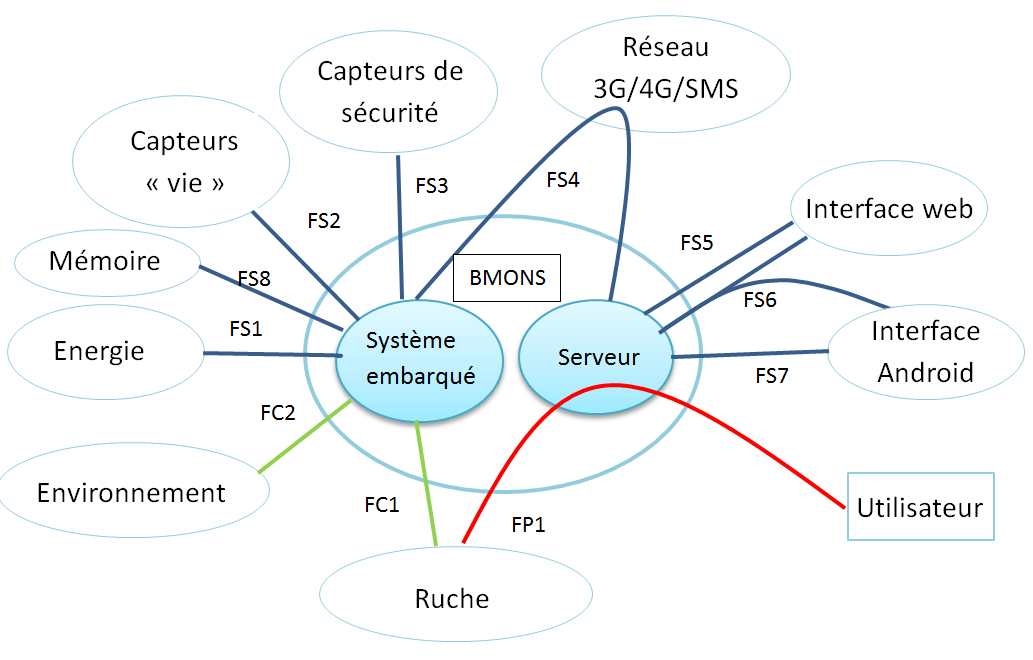
\includegraphics[scale=0.5]{pieuvre1.png}
\caption{\label{fig:diagpieuvre1} Diagramme pieuvre du système BMONS}
\end{figure}

\begin{figure}[h!]
\centering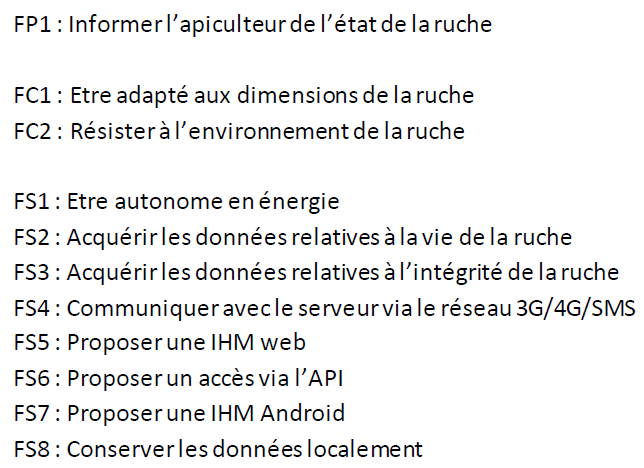
\includegraphics[scale=0.5]{pieuvre2.png}
\caption{\label{fig:diagpieuvre2} Légende diagramme pieuvre du système BMONS}
\end{figure}


\chapter{Spécification fonctionnelle  3 axes}

\section{Raffinement FAST}

Le diagramme FAST regroupe les fonctions principales, techniques et contraintes globales définies dans lors de 
l'établissement des exigences et après leur discussion avec le client. Ainsi, certaines exigences que nous avons préalablement établit ont été acceptée mais d'autres ont écartée comme l'analyse des odeurs dans la ruche jugée finalement trop compliquée à mettre en place et difficile à exploiter. D'autres exigences ont vu le jours après les échanges avec l'apiculteur ce qui est venus enrichir et compléter notre tableau des exigences. Le raffinement des trois types de fonctions en sous fonctions et les solutions techniques 
associées a celles-ci apparaissent également. Il a évolué au cours du projet en fonction des autres documents 
d'ingénierie système et des solutions techniques retenues. 
On peut voir la version finale du FAST sur la figure \ref{fig:fast}

\begin{figure}[h!]
\centering\includegraphics[scale=0.8]{FAST_BMONS.pdf}
\caption{\label{fig:fast} Diagramme FAST du système BMONS}
\end{figure}

\clearpage

\section{Spécification des données}

La spécification des données permet de mettre à jour les différentes grandeurs 
et unités intervenant dans notre système. Grâce à cela, nous savons exactement 
quel type de donnée traiter et comment convertir les données numériques de sortie des capteurs en grandeurs physiques facilement compréhensible pour l'apiculteur. Il faudra ensuite envoyer ces données traitées au serveur qui les stockera dans une base de données. Cette étude a aussi permis d'établir les alertes qu'il va falloir prévoir afin d'avertir le propriétaire de l'état de son rucher. Ces dernières seront aussi stockées sur le serveur qui viendront compléter l'historique de la ruche. Il est possible qu'une alerte soit envoyée après avoir effectué un recoupement d'informations Par exemple, pour alerter l'apiculteur d'un essaimage en cours, il est nécessaire de détecter une agitation dans la ruche (chant de la reine) grâce au microphone et une chute importante de la masse grâce à la balance. 

Il existera deux types d'alertes: les alertes actives qui préconiserons l'apiculteur à agir directement sur la ruche (par exemple lorsque le développement de la grappe est excentrée par rapport aux cadres) et des alertes passives qui encourageront le client à se rendre sur le serveur pour consulter les derniers relevés.   

L'axe Data comportant la spécification des messages, des évènements et des alarmes est fourni en annexe.
Le diagramme des données est décris dans la figure \ref{fig:donnees} 



\begin{figure}[h!]
\centering\includegraphics[scale=0.3]{diagFluxDonnees.jpg}
\caption{\label{fig:donnees} Diagramme d'activité du flux de données}
\end{figure}

\clearpage

\section{Modèle de Données}

Le modèle de données est une façon abstraite de représenter les données du système et de modéliser les informations contenus dans une base de données. Le modèle constitue des ensembles possèdent d'un nom et des attributs nommés. La  des relations est fait via des clés primaires (id, dans notre cas) et des clés étrangères.  

\ref{fig:UML} 



\begin{figure}[h!]
\centering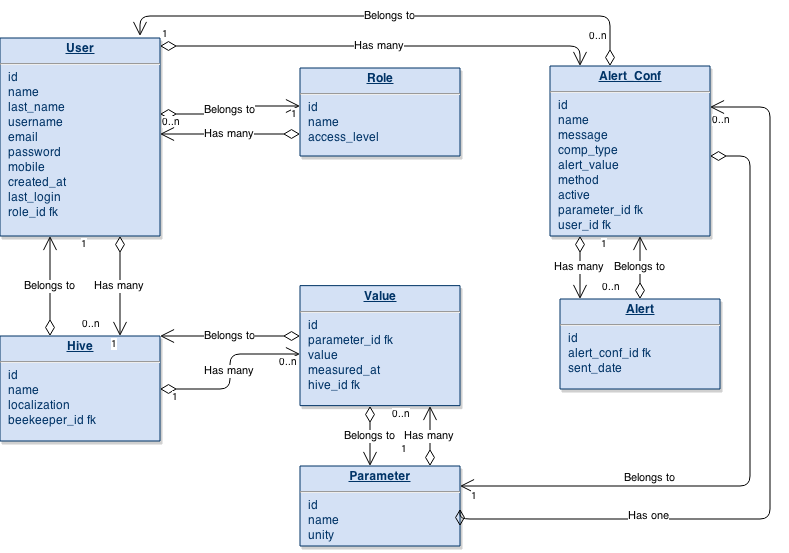
\includegraphics[scale=0.55]{UML.png}
\caption{\label{fig:UML} Modèle de données pour le système BMONS}
\end{figure}

\clearpage

\section{Spécification des comportements}

Nous allons ici décrire le fonctionnement de notre système. Il est résumé dans la figure \ref{fig:sp_comp}.

\begin{figure}[h!]
\centering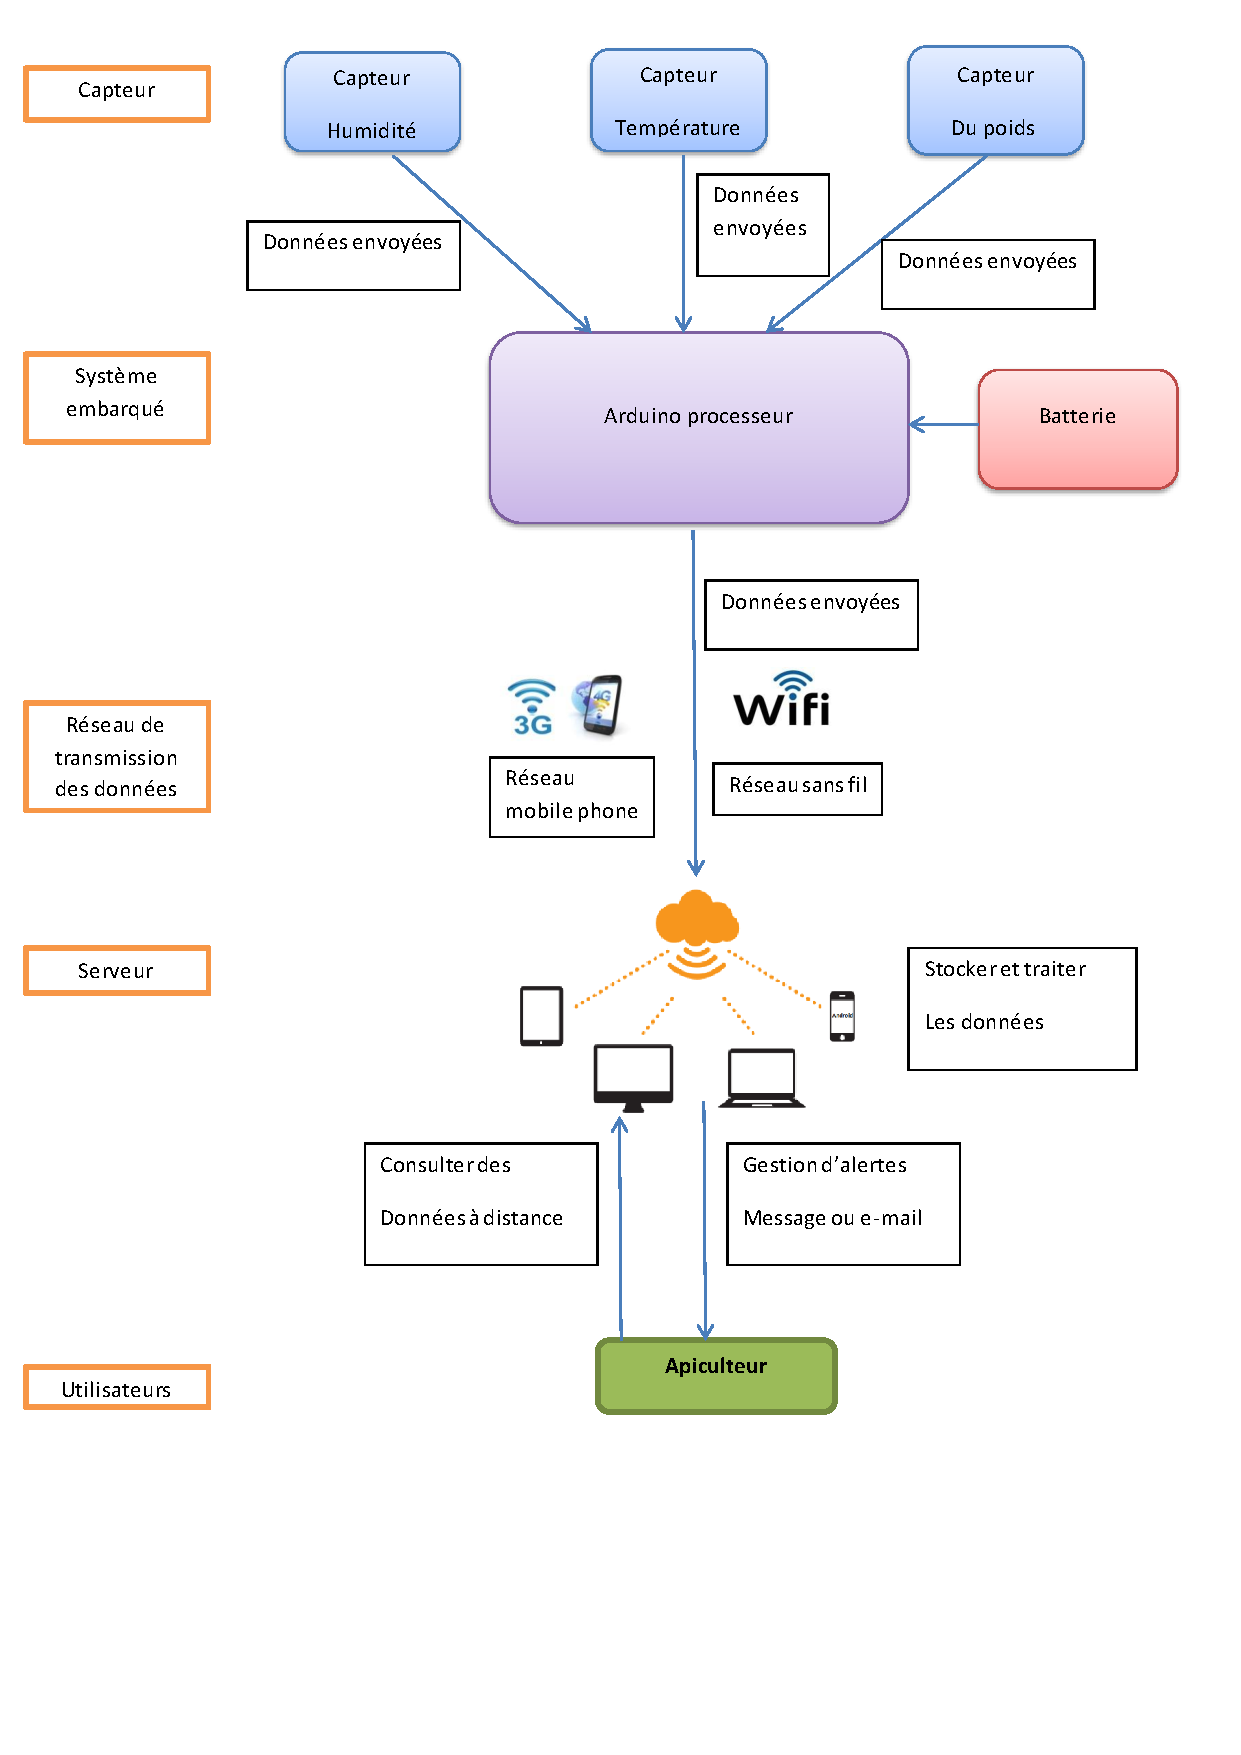
\includegraphics[scale=0.5]{specif_comp.pdf}
\caption{\label{fig:sp_comp} Diagramme de spécification des comportements}
\end{figure}

Les capteurs mesurent plusieurs paramètres internes à la ruche : l'humidité, la température et le poids de la ruche. Les données sont ensuite transmises au système embarqué. Dès que le système embarqué les reçoit, il traite les données, sélectionne celles qui sont valides et les envoi au serveur soit par le réseau sans fil (2G ou 3G), soit par le réseau téléphone si besoin. Une fois que le serveur reçoit les données, elles sont traitées et stockées dans une base de données sécurisée. Une représentation sous forme de graphiques permet une vision pratique et exploitable des informations par l'apiculteur.

Quand les mesures effectuées dépassent certain critères, par exemple, si la température est plus élevée que la température maximum pour la ruche, le serveur va générer un alerte qui sera envoyée à l'utilisateur, c’est-à-dire l'apiculteur, par SMS ou par e-mail. Par ailleurs, les apiculteurs peuvent consulter l’état de la ruche à distance afin de bien gérer la productivité de la ruche ou de limiter les situations problématiques. 

La spécification du comportement ce fait également grace aux diagrammes de séquence. Ces diagrammes expliquent précisément comment les different parties du systeme interagisent dans le but d'executer une action. Ils détail l'ordre des actions ainsi que leur nature et leur durée d'execussion. A ce jour 5 diagrames de séquence ont été réalisé ils concernent l'action de récuperation de la mémoire flash, l'analyse des information par le serveur, le service permetant à l'apiculteur d'avertir le serveur d'une intervention sur une ruche, la fonction permetant la configuratiion des alertes et l'action de connecxion d'un apiculteur à son compte.
\begin{figure}[h!]
\centering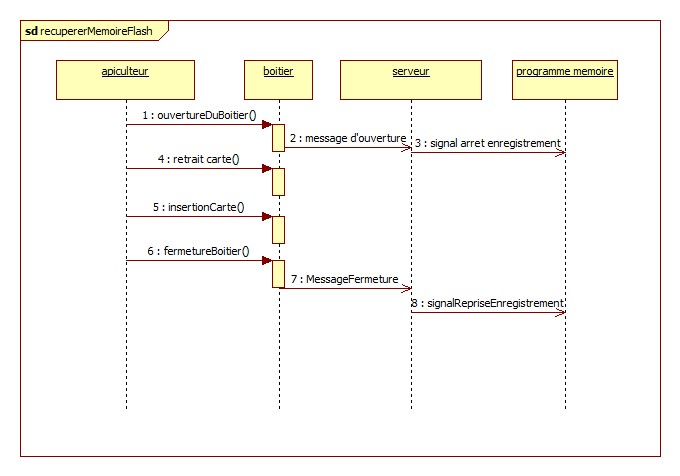
\includegraphics[scale=0.7]{recupererMemoireFlash.jpg}
\caption{\label{fig:sp_comp} Diagramme de spécification des comportements}
\end{figure}
\begin{figure}[h!]
\centering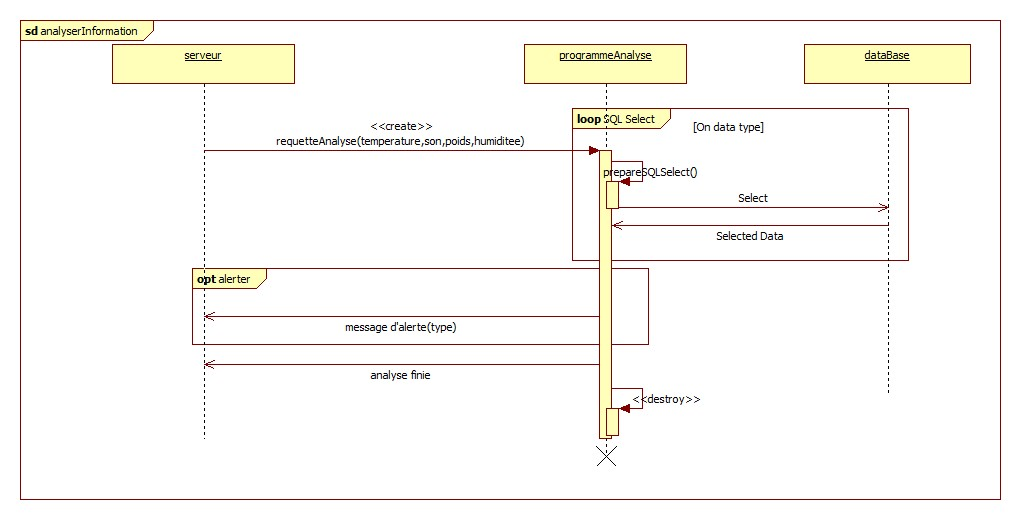
\includegraphics[scale=0.7]{analyserInformation.jpg}
\caption{\label{fig:sp_comp} Diagramme de spécification des comportements}
\end{figure}
\begin{figure}[h!]
\centering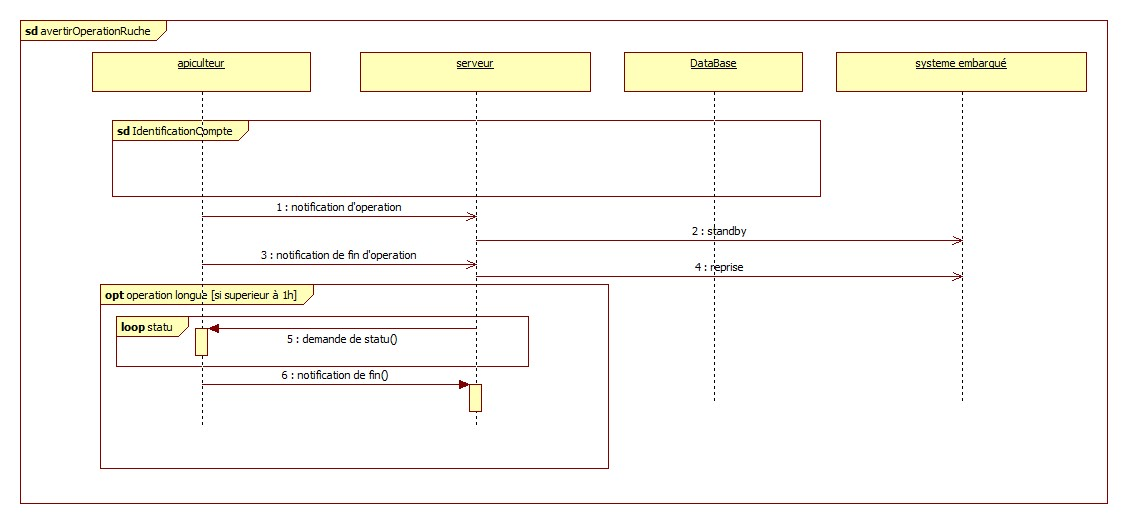
\includegraphics[scale=0.7]{avertirOperationRuche.jpg}
\caption{\label{fig:sp_comp} Diagramme de spécification des comportements}
\end{figure}
\begin{figure}[h!]
\centering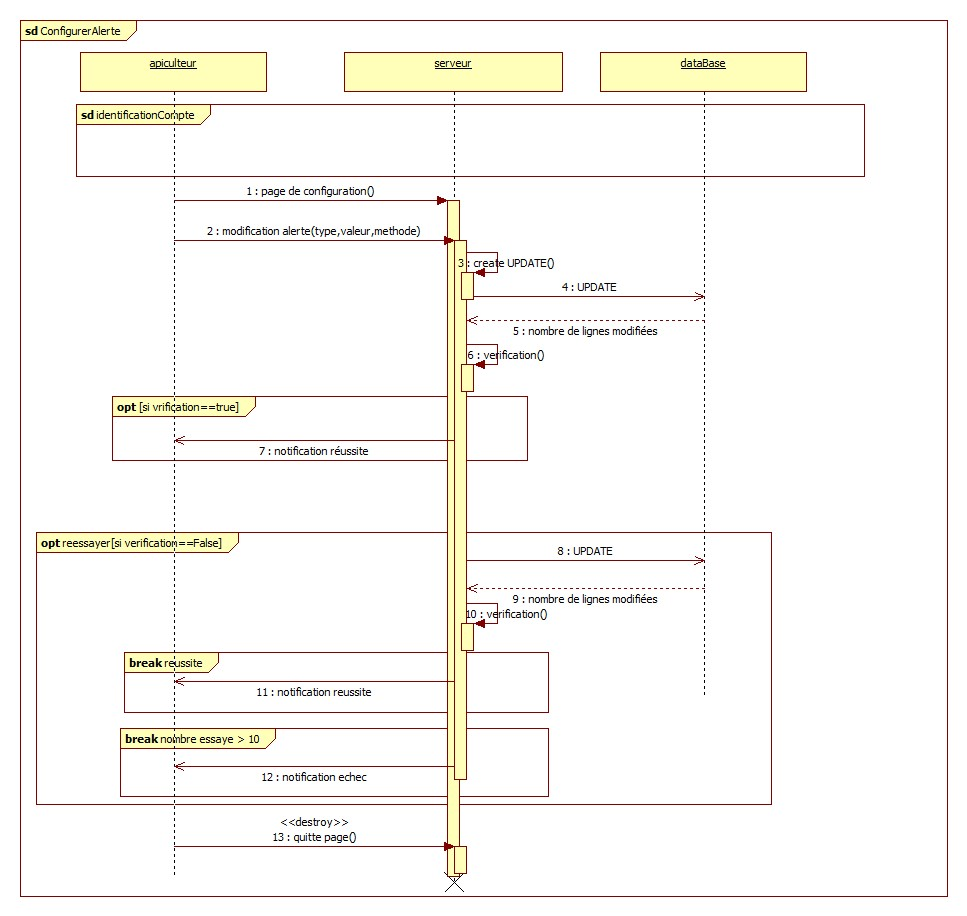
\includegraphics[scale=0.7]{configurerAlerte.jpg}
\caption{\label{fig:sp_comp} Diagramme de spécification des comportements}
\end{figure}
\begin{figure}[h!]
\centering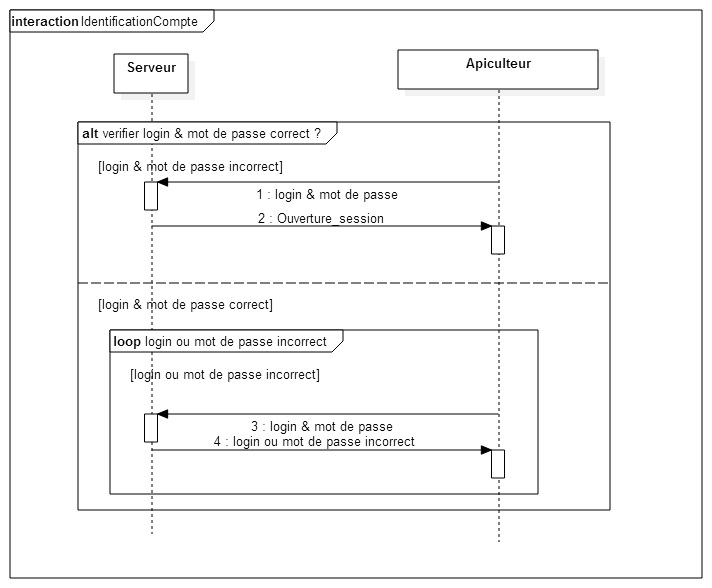
\includegraphics[scale=0.7]{IdentificationCompte.jpg}
\caption{\label{fig:sp_comp} Diagramme de spécification des comportements}
\end{figure}
\pagebreak

\chapter{Architecture fonctionnelle}

L'étude de la spécification fonctionnelle trois axes a permis d'établir l'architecture fonctionnelle du système qui est représentée sur la figure \ref{fig:anaFonc}.
Ce schéma résume les interactions entre chaque partie: Bee Monitor qui regroupe l'ensemble des capteurs, la carte Arduino ainsi que la carte SSD pour l'enregistrement local des données, le module de transmission et le système d'alimentation rendant notre projet autonome en énergie et le serveur. Chaque acteur interagissant avec le système y sont également représentés: Les abeilles/ruche, l'apiculteur et l'environnement.   
  

\begin{figure}[h]
\centering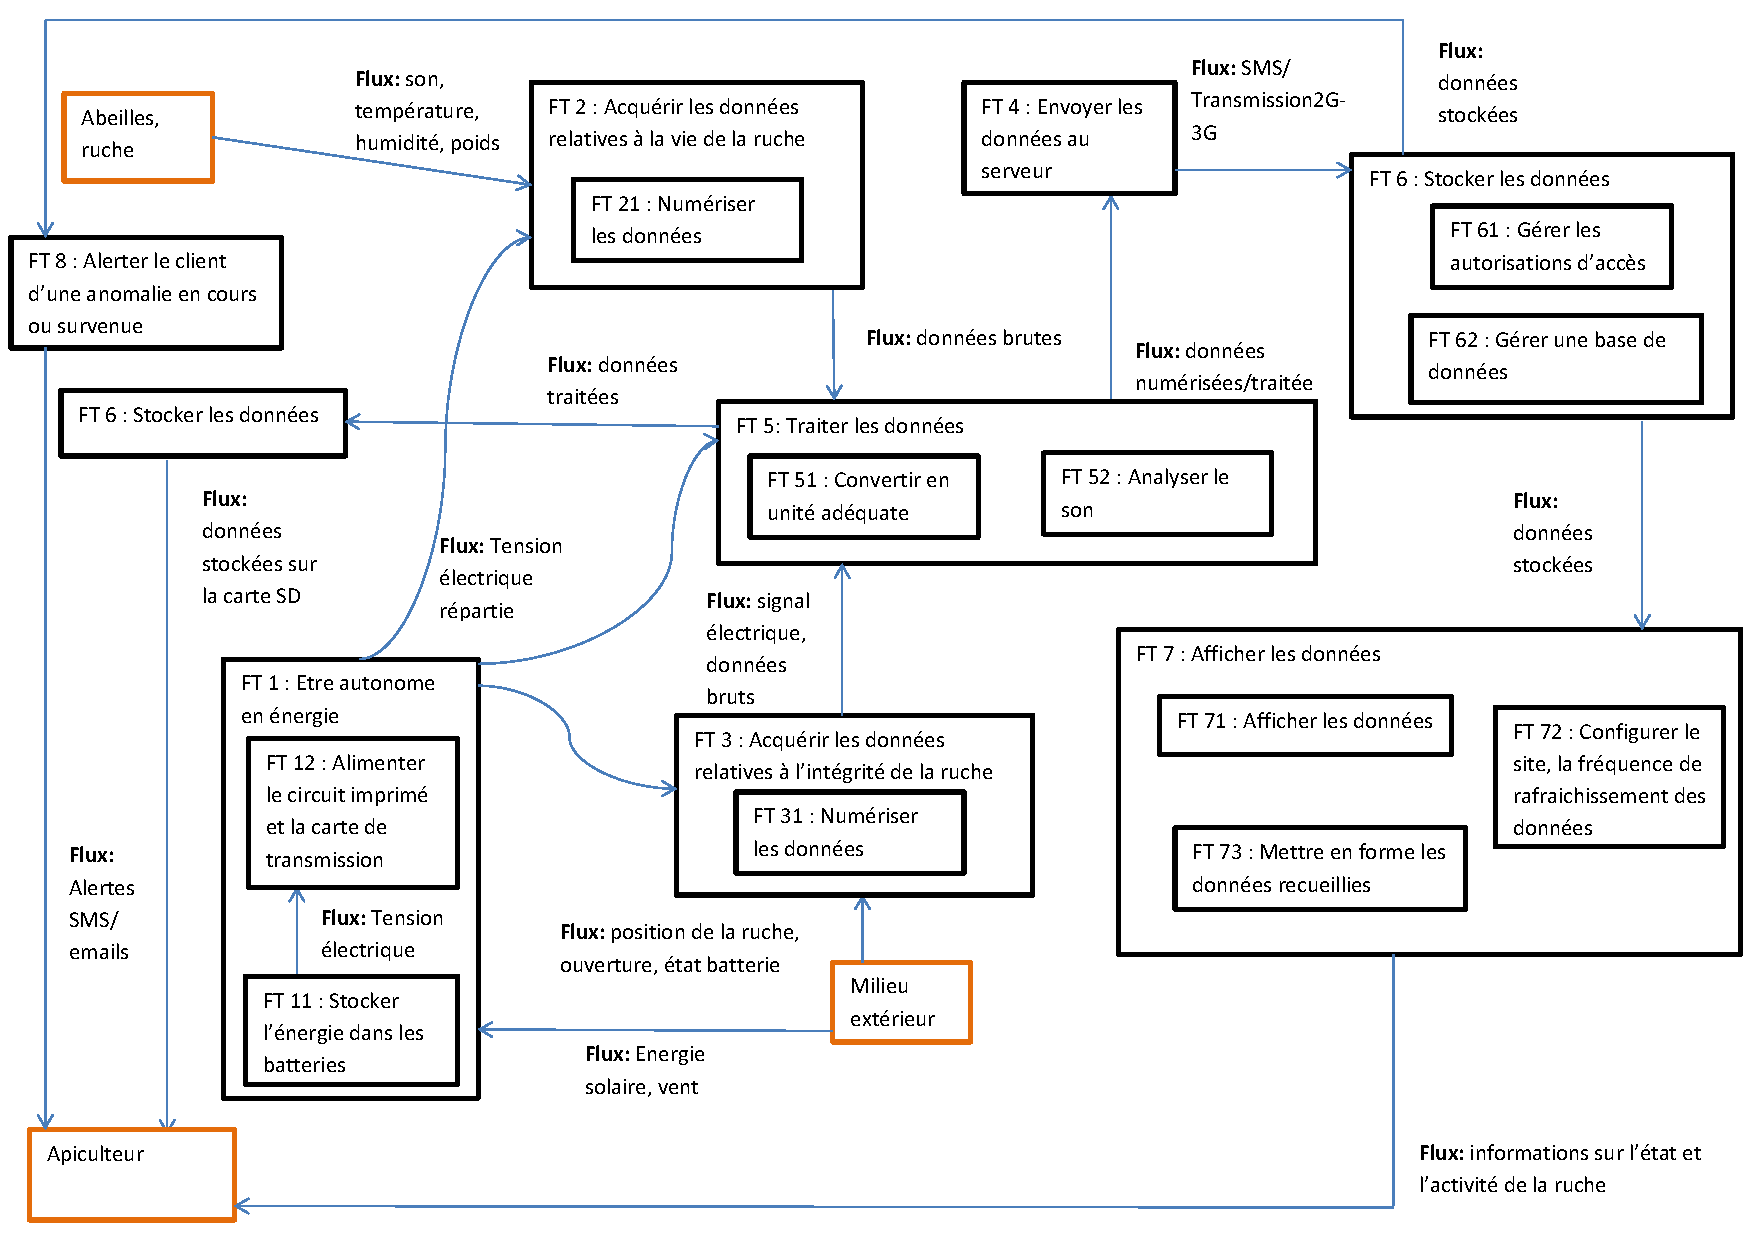
\includegraphics[scale=0.5]{analyseFonctionelle1.pdf}
\caption{\label{fig:anaFonc} Architecture fonctionnelle}
\end{figure}    

